\chapter{Theorie}
	
	\section{DeepLab}
		DeepLab ist ein von Google entwickeltes, 2015  in \cite{DeepLab1} vorgestelltes Modell f�r semantische Segmentierung. Bei der in \cite{DeepLab2} vorgestellten Methode wird ein Deep Convolutional Neural Network (DCNN) zum Erzeugen einer Score Map benutzt, die anschlie�end mit einem Conditional Random Field (CRF) zur endg�ltigen Ausgabe weiterverarbeitet wird. Das Verfahren wird in Abbildung \ref{fig:DeepLabAblauf} grob dargestellt.
		
		\begin{figure}
			\centering
			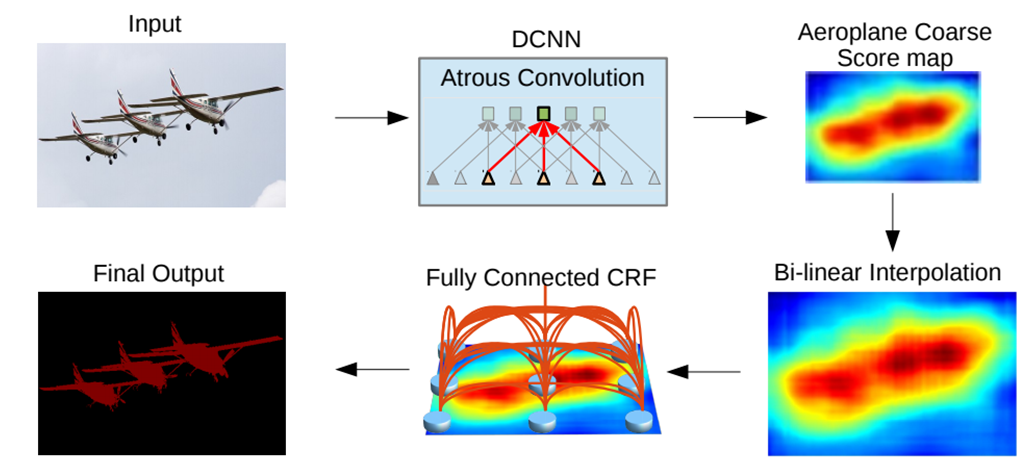
\includegraphics[width = 0.9\linewidth]{img/DeepLabAblauf.png}
			\caption{Grunds�tzliche Funktionsweise von DeepLab}
			\label{fig:DeepLabAblauf}
		\end{figure}  
		\subsection{Deep Convolutional Neural Networks f�r Semantische Segmentierung}
			\subsubsection{Convolutional Neural Networks}
				
			\subsubsection{Anpassungen f�r Semantische Segmentierung}
				Klassische DCNNs haben Eigenschaften, die sie f�r die Verwendung zur Bildsegmentierung nicht ideal machen. 
				\begin{itemize}
					\item Der Einsatz von Downsampling f�hrt zu verringerter Aufl�sung, die bei Klassifizierungsaufgaben nicht ins Gewicht f�llt, f�r die Segmentierung aber essentiell ist. 
					\item Neuronale Netze sind in der Regel gut geeignet, um Objekte unterschiedlicher Gr��e zu erkennen, wenn solche in der Lernphase pr�sentiert werden. Die Eigenschaften der Faltung, insbesondere dem begrenzten Sichtbereich beim Berechnen eines einzelnen Pixels ist allerdings f�r diese Problematik ung�nstig.
					\item Der wiederholte Einsatz von Convolutional Layers f�hren zu einem Verlust an Ortsinformation. Infolgedessen produzieren DCNNs bei Segmentierungsaufgaben verschwommene, oft verrauschte Ergebnisse ohne klare Kanten.
				\end{itemize}
			
			Um diese Probleme zu l�sen erh�lt das von DeepLab verwendete DCNN einige Anpassungen. Zun�chst werden alle Fully Connected Layers durch Convolutional Layers ersetzt, um ein Fully Convolutional Network zu bilden. 
			Noch dazu wird anstatt von Pooling Layers in den unteren Schichten Atrous Convolution eingesetzt, womit die Aufl�sung der Ausgabe erh�ht wird. In den h�heren Schichten werden auch hier Pooling Layers eingesetzt, um Speicherbedarf und Rechenzeit zu verbessern. 
			Um die Gr��eninvarianz zu verbessern wird bei den unteren Schichten Atrous Spatial Pyramid Pooling verwendet.
			
		\subsection{Atrous Convolution}
			Atrous Convolution, auch Dilated Convolution genannt, beschreibt eine Technik bei der eine Matrix mit einem sp�rlich best�ckten Kernel gefaltet wird, wie in Abbildung \ref{fig:AtrousConv} illustriert.
			
				\begin{figure}
					\centering
					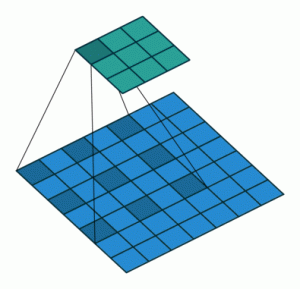
\includegraphics[]{img/AtrousConv.png}
					\caption{Prinzip von Atrous Convolution}
					\label{fig:AtrousConv}
				\end{figure} 
			Die Abst�nde der zu ber�cksichtigenden Werte in der Matrix wird dabei durch die s.g. Dilation Rate bzw. Erweiterungsrate (kurz Rate) festgelegt. Das Tats�chliche Sichtfeld des Filters wird also festgelegt durch die Gr��e des Kernels und die Rate bestimmt.\\ ein Filter mit einem Kernel der Gr��e 3x3 und einer Rate von 2, was dem Einf�gen einer leeren Zeilen und Spalte zwischen den Werten entspricht, hat demnach ein Sichtfeld der Gr��e 5x5.
			Dadurch wird das effektive Sichtfeld des Filters erh�ht und es kann eine h�here Aufl�sung bei gleichen Rechenaufwand erreicht werden. Die Vorteile der Verwendung von Atrous Convolution f�r Bildsegmentierung sind in Abbildung \ref{fig:AtrousConvRes} dargestellt.
				\begin{figure}
					\centering
					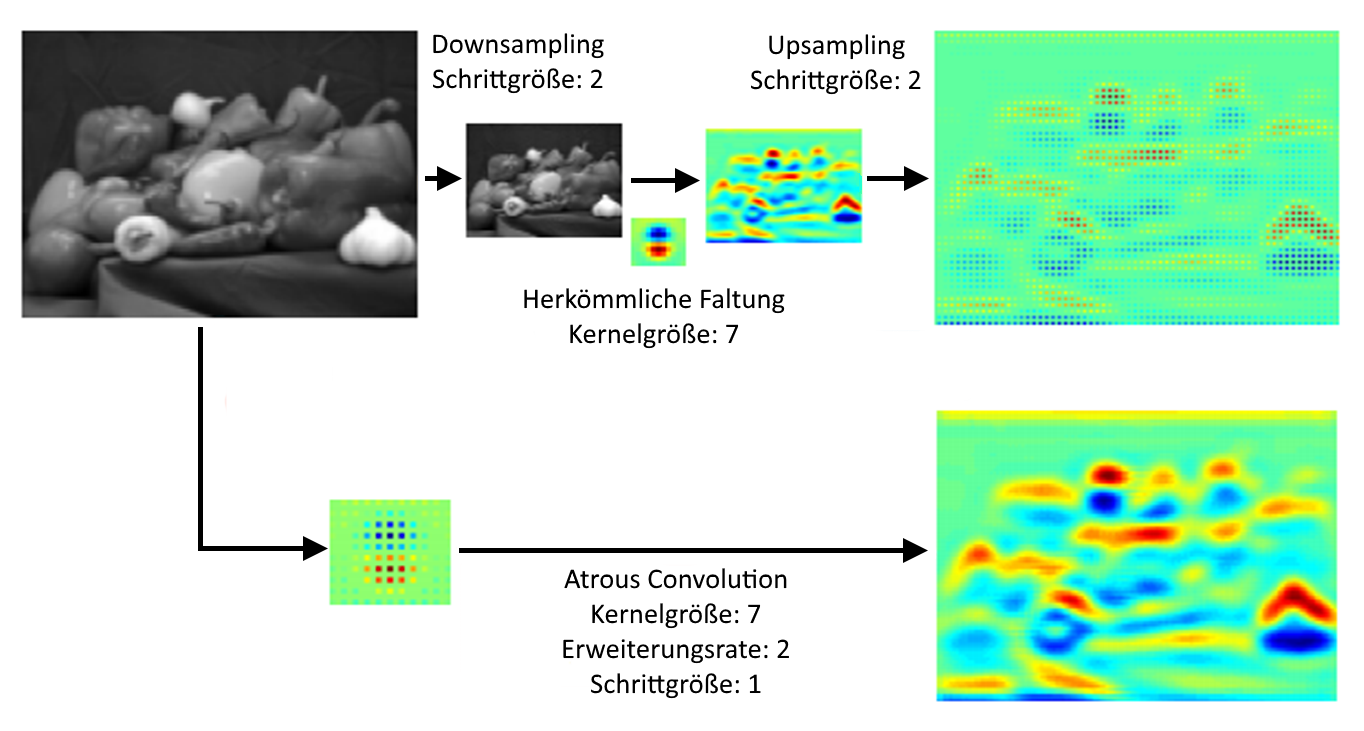
\includegraphics[width = 0.9\linewidth]{img/AtrousConvRes.png}
					\caption{Beispielhaft dargestellte Vorteile von Atrous Convolution}
					\label{fig:AtrousConvRes}
				\end{figure} 
		
		\subsection{Atrous Spatial Pyramid Pooling}
			Beim Atrous Spatial Pyramid Pooling werden mehrere parallele Convolutional Layers, die Atrous Convolutional Layers mit unterschiedlicher Rate verwenden, in das DCNN eingebaut. Das Prinzip ist in Abbildung \ref{fig:PyramPooling} dargestellt.\\
			Durch dieses Vorgehen soll Gr��eninvarianz erreicht werden.
			
				\begin{figure}
					\centering
					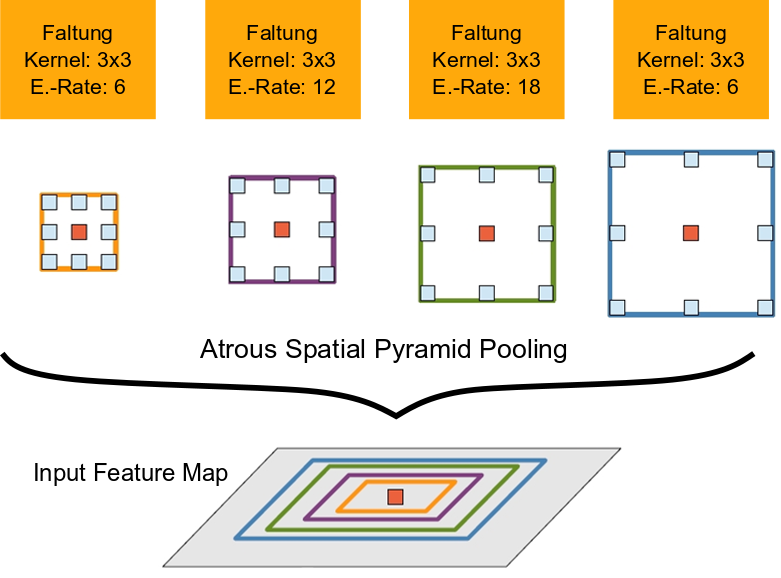
\includegraphics[width = 0.9\linewidth]{img/PyramPooling.png}
					\caption{Beispielhaft dargestellte Vorteile von Atrous Convolution}
					\label{fig:PyramPooling}
				\end{figure} 
		\subsection{Fully-Connected Conditional Random Fields}
		\subsection{Residual Networks}
	\section{Kamerakalibrierung}
		